\documentclass{article}
\usepackage[utf8]{inputenc}
\usepackage[usenames,dvipsnames]{color}
\usepackage{tikz}
\usetikzlibrary{mindmap, trees}

\begin{document}
\begin{figure}
\caption{Ejemplo de estructura IMRAD en los documentos científicos y académicos}
\label{fig.mapa.mental}
\begin{center}
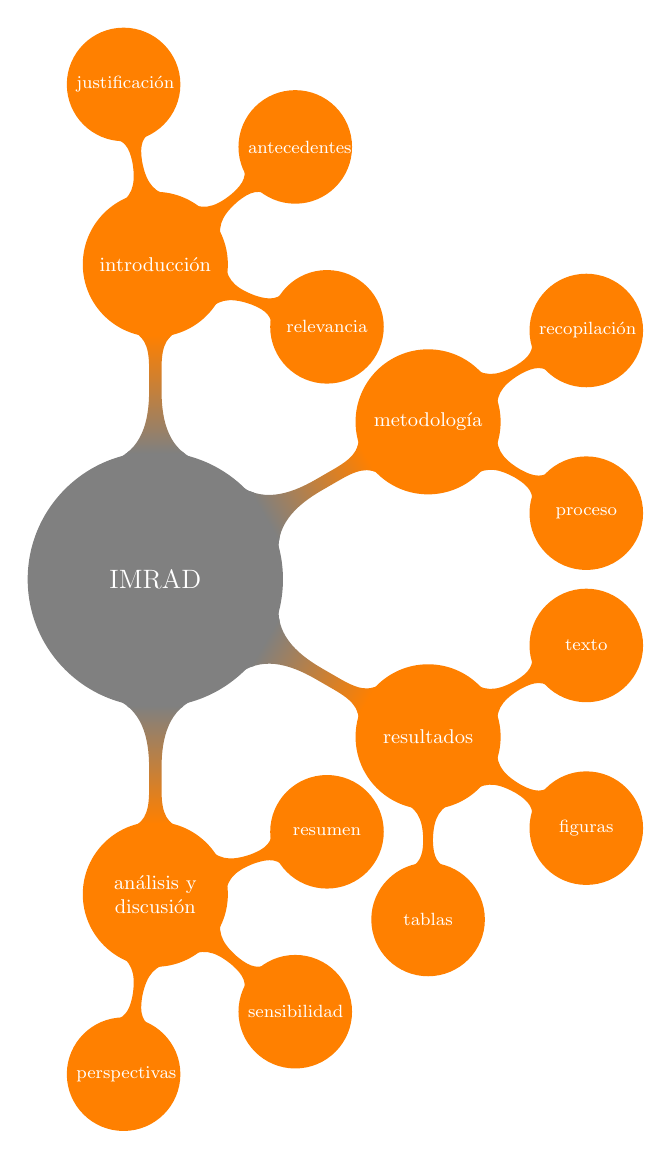
\begin{tikzpicture}[thick, scale=0.8, every node/.style={scale=0.8}]
\path[mindmap, concept color=gray, text=white]
    node[concept] {IMRAD} [clockwise from=90]
      child[concept color=orange] {
        node[concept] {introducci{\'o}n} [clockwise from=100]
          child { node[concept] {justificaci{\'o}n} }
          child { node[concept] {antecedentes} }
          child { node[concept] {relevancia} }                            
                                  }
      child[concept color=orange] {
        node[concept] {metodolog{\'i}a} [clockwise from=30]
          child { node[concept] {recopilaci{\'o}n} }
          child { node[concept] {proceso } }
                                  }
      child[concept color=orange] {
        node[concept] {resultados} [clockwise from=30]
          child { node[concept] {texto} }
          child { node[concept] {figuras} }
          child { node[concept] {tablas} }
                                  }
      child[concept color=orange] {
        node[concept] {an{\'a}lisis y discusi{\'o}n}  [clockwise from=20]
          child { node[concept] {resumen} }
          child { node[concept] {sensibilidad} }
          child { node[concept] {perspectivas} }
                                  };
\end{tikzpicture}
\end{center}
\rule{\textwidth}{.1pt}
\noindent \footnotesize Ejemplo de estructura de un documento científico, conocida como IMRAD (Introducción, Metodología, Resultados, Análisis y discusión).
\end{figure}

\end{document}
